\documentclass[AutoFakeBold,AutoFakeSlant]{beamer}
\usepackage{ctex}
\usepackage{hyperref}
\usepackage[defaultsans]{droidsans}
\usepackage{fontspec}
\usepackage{newtxmath}
\usepackage{latexsym,amsmath,xcolor,multicol,booktabs,calligra}
\usepackage{graphicx,tabularx,multirow,makecell}
\usepackage{tikz}
\usetikzlibrary{arrows.meta,positioning}
\usetheme{Madrid}
\usecolortheme{default}
\setbeamertemplate{navigation symbols}{}
\setbeamertemplate{footline}[frame number]
\graphicspath{{./figures_lab4/}}

\author{李禹江，张博涵，蒋兴宇}
\title{Android 隐私检测系统\\Lab4 系统设计与实验汇报}
\subtitle{证据驱动的知情权、同意权、访问权自动化审计}
\institute{我的刀盾队}
\date{2026-05-25}

\begin{document}
\kaishu

\begin{frame}
    \titlepage
\end{frame}

\begin{frame}
    \frametitle{目录}
    \tableofcontents
\end{frame}

\section{背景与目标}

\begin{frame}
    \frametitle{研究背景}
    \small
    \begin{itemize}
        \item 课程/课题 \textbf{Lab4} 要求从「文本承诺」延伸到「技术可验证」：政策声明是否与真实采集、开关控制、副本导出一致。
        \item 早期方案以 \textbf{LLM 主导} 判断为主；现实现以 \textbf{证据包 + 规则引擎 + 法律知识库} 为主，因此本次实验中 LLM 仅保留在政策句级审计历史链路。
        \item 本汇报对齐 \textbf{系统设计 Lab4}：总体架构、模块划分、数据流、三项权利实验与局限说明。
    \end{itemize}
\end{frame}

\begin{frame}
    \frametitle{Lab4 三项权利与评价维度}
    \small
    \begin{tabularx}{\textwidth}{|l|X|l|}
        \hline
        \textbf{维度} & \textbf{核心问题} & \textbf{本批结果} \\
        \hline
        Lab4-1 知情权 & 政策声明 PII 类型 vs 多源观测是否一致 & \textbf{9/9} 成功 \\
        \hline
        Lab4-2 同意权 & 关闭隐私开关前后 Frida 命中是否停止 & 暂未有效实证 \\
        \hline
        Lab4-3 访问权 & 声明、运行时与「副本」字段是否覆盖 & 流水线 \textbf{9/9}；覆盖率均为 0 \\
        \hline
    \end{tabularx}
    \vspace{0.4em}
    \scriptsize
    Job ID 前缀：\texttt{exp\_stage3\_20260525}；样本 9 App（\texttt{apps\_lab4\_batch.txt}）。
\end{frame}

\section{系统总体设计}

\begin{frame}
    \frametitle{系统总体架构}
    \scriptsize
    \centering
    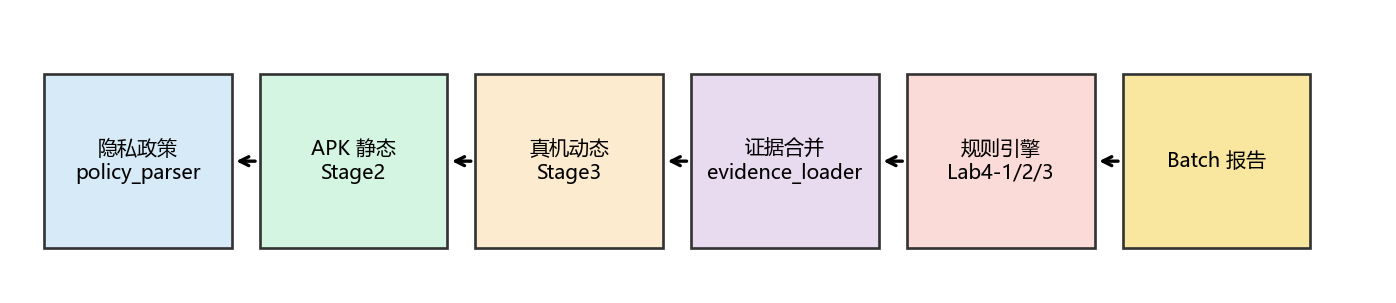
\includegraphics[width=0.98\linewidth]{fig_pipeline_overview.png}
    \vspace{0.3em}
    \begin{itemize}
        \item \textbf{输入}：\texttt{input/pii\_text/<App>.txt}、APK（可选）、\texttt{oldsrc} 历史 JSON。
        \item \textbf{Stage2}：Exodus + Androguard $\rightarrow$ \texttt{static\_evidence.json}。
        \item \textbf{Stage3}：Appium 政策路径 + Frida $\rightarrow$ \texttt{dynamic\_evidence.json}。
        \item \textbf{合并}：\texttt{evidence\_loader} + \texttt{privacy\_knowledgebase} $\rightarrow$ \texttt{lab4\_1\_evidence/<App>.json}。
        \item \textbf{输出}：\texttt{lab4\_1/2/3} 报告 + batch summary + manifest。
    \end{itemize}
\end{frame}

\begin{frame}
    \frametitle{端到端 Pipeline（程序管线）}
    \small
    \begin{enumerate}
        \item \textbf{政策解析}：\texttt{policy\_parser} $\rightarrow$ \texttt{declared\_pii[]}
        \item \textbf{静态分析}：\texttt{stage2\_static}（Exodus + Androguard）
        \item \textbf{动态取证}：\texttt{stage3\_dynamic}（\texttt{appium\_runner} + Frida hooks）
        \item \textbf{证据导入}：\texttt{import-oldsrc}、\texttt{build-evidence-bundles}
        \item \textbf{知识库}：\texttt{kb-build} $\rightarrow$ \texttt{feasible\_evidence[]}
        \item \textbf{权利审计}：\texttt{lab4-1-audit} / \texttt{lab4-2-audit} / \texttt{lab4-3-audit}
        \item \textbf{批量}：\texttt{batch} + \texttt{--retry} + 日志归档
    \end{enumerate}
    \vspace{0.2em}
    \scriptsize
    统一入口：\texttt{python -m privacy\_audit.cli}（工作目录 \texttt{project/src}）。
\end{frame}

\begin{frame}
    \frametitle{核心模块划分}
    \small
    \begin{columns}[T]
        \begin{column}{0.48\textwidth}
            \textbf{ingestion}
            \begin{itemize}
                \item \texttt{policy\_parser}
                \item \texttt{evidence\_loader}
                \item \texttt{privacy\_knowledgebase}
            \end{itemize}
            \textbf{analyzers}
            \begin{itemize}
                \item \texttt{compare\_engine}（Lab4-1）
                \item \texttt{consent\_compare}（Lab4-2）
                \item \texttt{access\_compare}（Lab4-3）
            \end{itemize}
        \end{column}
        \begin{column}{0.48\textwidth}
            \textbf{dynamic}
            \begin{itemize}
                \item \texttt{appium\_runner}
                \item \texttt{element\_tap}（Tab/齿轮/头像）
                \item \texttt{frida\_collector}
            \end{itemize}
            \textbf{reporting}
            \begin{itemize}
                \item \texttt{lab4\_1\_report} 等
                \item \texttt{batch} / manifest
            \end{itemize}
        \end{column}
    \end{columns}
\end{frame}

\begin{frame}
    \frametitle{设计原则：与早期计划的差异}
    \small
    \begin{tabularx}{\textwidth}{|l|X|X|}
        \hline
        \textbf{方面} & \textbf{早期（plan / 开发计划）} & \textbf{现实现} \\
        \hline
        判定主体 & LLM 直接输出 verdict & 规则引擎 + 可溯源 provenance \\
        \hline
        动态测试 & 泛化 UI 探索 & 政策路径驱动 + 分 App 适配 \\
        \hline
        证据来源 & 单一通道 & static + dynamic + oldsrc + KB \\
        \hline
        工程形态 & 脚本分散 & 统一 CLI + batch + job id \\
        \hline
    \end{tabularx}
\end{frame}

\begin{frame}
    \frametitle{Lab4-1 判定逻辑（知情权）}
    \scriptsize
    \begin{itemize}
        \item 输入：\texttt{declared\_pii[]}（政策）与 \texttt{observed\_pii[]}（合并证据）。
        \item 输出 verdict：\texttt{consistent}、\texttt{inconsistent\_high\_risk}、\texttt{declared\_not\_observed}、KB 相关类型等。
        \item 每条结论附带 \texttt{sources[]} / \texttt{provenance}，便于答辩追问「证据从哪来」。
    \end{itemize}
    \vspace{0.2em}
    \centering
    \begin{tikzpicture}[
        node distance=4mm and 5mm,
        box/.style={draw, rounded corners, align=center, minimum width=2.0cm, minimum height=7mm, font=\tiny},
        arr/.style={-{Latex[length=1.4mm]}, thick},
    ]
        \node[box, fill=blue!10] (d) {政策声明};
        \node[box, fill=green!12, right=of d] (o) {多源观测};
        \node[box, fill=orange!14, right=of o] (c) {compare\_engine};
        \node[box, fill=violet!10, below=of c] (r) {Lab4-1 报告};
        \draw[arr] (d) -- (c);
        \draw[arr] (o) -- (c);
        \draw[arr] (c) -- (r);
    \end{tikzpicture}
\end{frame}

\section{实验设计}

\begin{frame}
    \frametitle{实验环境与样本}
    \small
    \begin{itemize}
        \item \textbf{环境}：Windows + MuMu（ADB）+ Appium \texttt{4723} + Frida（版本需与 \texttt{frida-server} 匹配）。
        \item \textbf{样本}：Keep、小红书、支付宝、LOFTER、智联招聘、世纪佳缘、好大夫医生版、东方财富、小荷健康。
        \item \textbf{包名映射}：\texttt{input/app\_packages.json}（小荷：\texttt{com.lvsongguo}）。
        \item \textbf{批次}：\texttt{exp\_stage3\_20260525\_lab4\_1/2/3}。
    \end{itemize}
\end{frame}

\begin{frame}
    \frametitle{Stage3 动态取证}
    \small
    \begin{itemize}
        \item 命令：\texttt{stage3-dynamic --app <名> --package <包> --policy-txt ...}
        \item 产物：\texttt{output/stage3\_dynamic\_real/<App>/dynamic\_evidence.json}、截图、\texttt{stage3\_run.log}。
        \item \textbf{共性}：9 App 均有产物；\texttt{frida\_runtime\_events = 0}（仅 \texttt{hook\_loaded} 登记）。
        \item Lab4-1 的 \texttt{observed\_pii} 主要来自 static、oldsrc、legacy、KB，\textbf{不能}全部表述为本次 Frida 实测。
    \end{itemize}
\end{frame}

\begin{frame}
    \frametitle{分 App UI 自动化要点}
    \scriptsize
    \begin{tabularx}{\textwidth}{|l|X|}
        \hline
        \textbf{App} & \textbf{要点} \\
        \hline
        世纪佳缘 & 底部 Tab 文案为 \texttt{" 我 "}（含空格）；按 bounds 点最右 Tab，避免误点「推荐」 \\
        \hline
        小荷健康 & 设置无文字；UserPage \textbf{右上角最右侧}齿轮为设置（左侧为扫一扫） \\
        \hline
        支付宝 & 需精确匹配「我的」等文案，避免宽泛「我」 \\
        \hline
        其他 & 政策路径 token + \texttt{element\_tap} 关键词/头像/齿轮兜底 \\
        \hline
    \end{tabularx}
\end{frame}

\section{实验结果}

\begin{frame}
    \frametitle{批量任务完成情况}
    \centering
    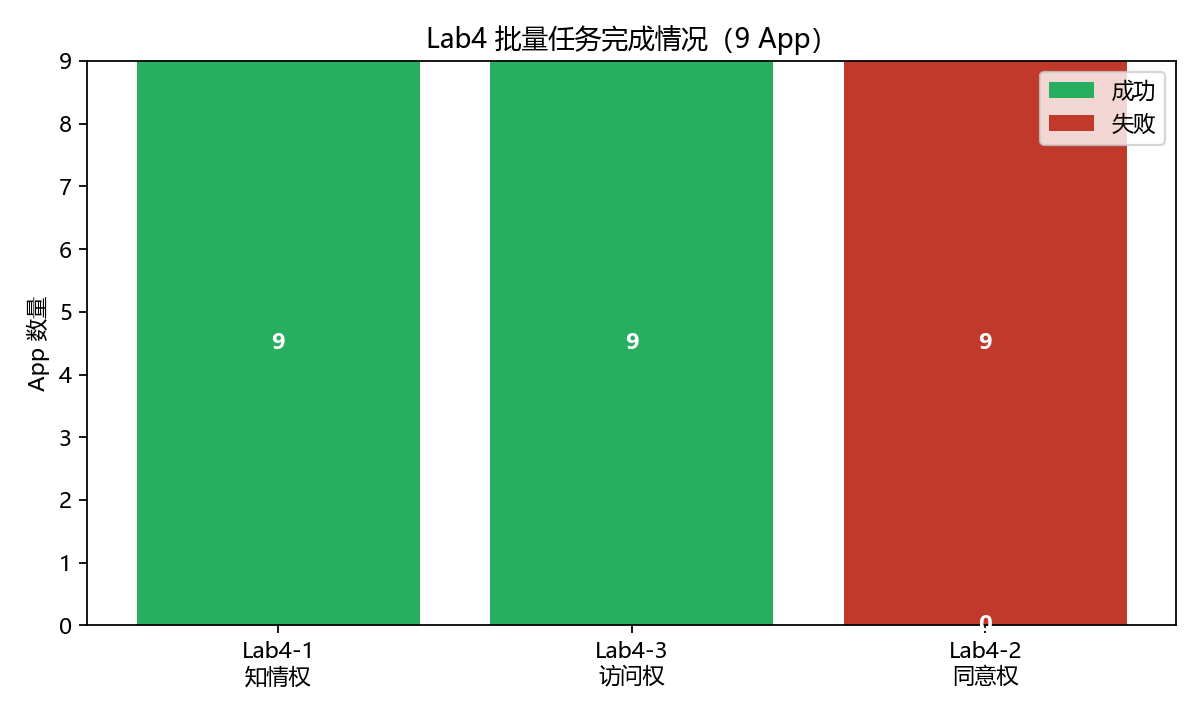
\includegraphics[width=0.82\linewidth]{fig_lab4_batch_status.png}
    \vspace{0.3em}
    \scriptsize
    Lab4-1、Lab4-3 程序批量 \textbf{9/9 成功}；Lab4-2 因无有效运行时前后对比，报告均为 \texttt{report\_status\_failed}。
\end{frame}

\begin{frame}
    \frametitle{Lab4-1 全样本合计（9 App）}
    \small
    \begin{tabular}{|l|r|}
        \hline
        \textbf{Verdict} & \textbf{条数} \\
        \hline
        consistent & 90 \\
        \hline
        inconsistent\_high\_risk & 41 \\
        \hline
        declared\_not\_observed & 6 \\
        \hline
    \end{tabular}
    \vspace{0.5em}
    \begin{itemize}
        \item \textbf{consistent}：政策声明且多源证据可支撑。
        \item \textbf{inconsistent\_high\_risk}：证据观测到但政策未充分声明（答辩可重点展开）。
        \item \textbf{declared\_not\_observed}：政策声明但当前证据链未观测到。
    \end{itemize}
\end{frame}

\begin{frame}
    \frametitle{Lab4-1：政策声明 vs 合并观测}
    \centering
    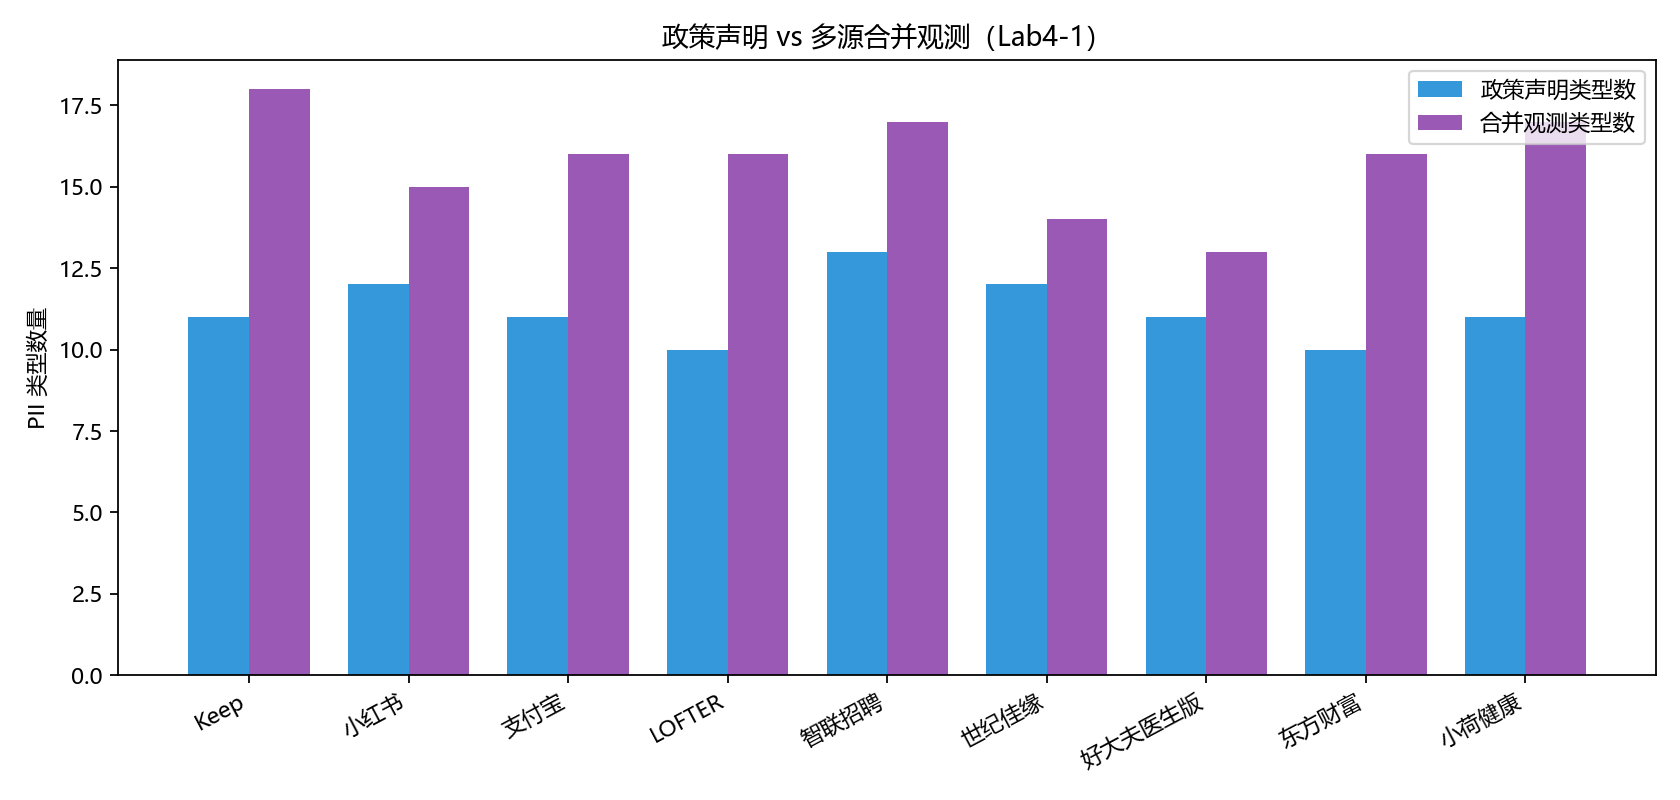
\includegraphics[width=0.95\linewidth]{fig_lab41_declared_observed.png}
\end{frame}

\begin{frame}
    \frametitle{Lab4-1：分应用 Verdict 分布}
    \centering
    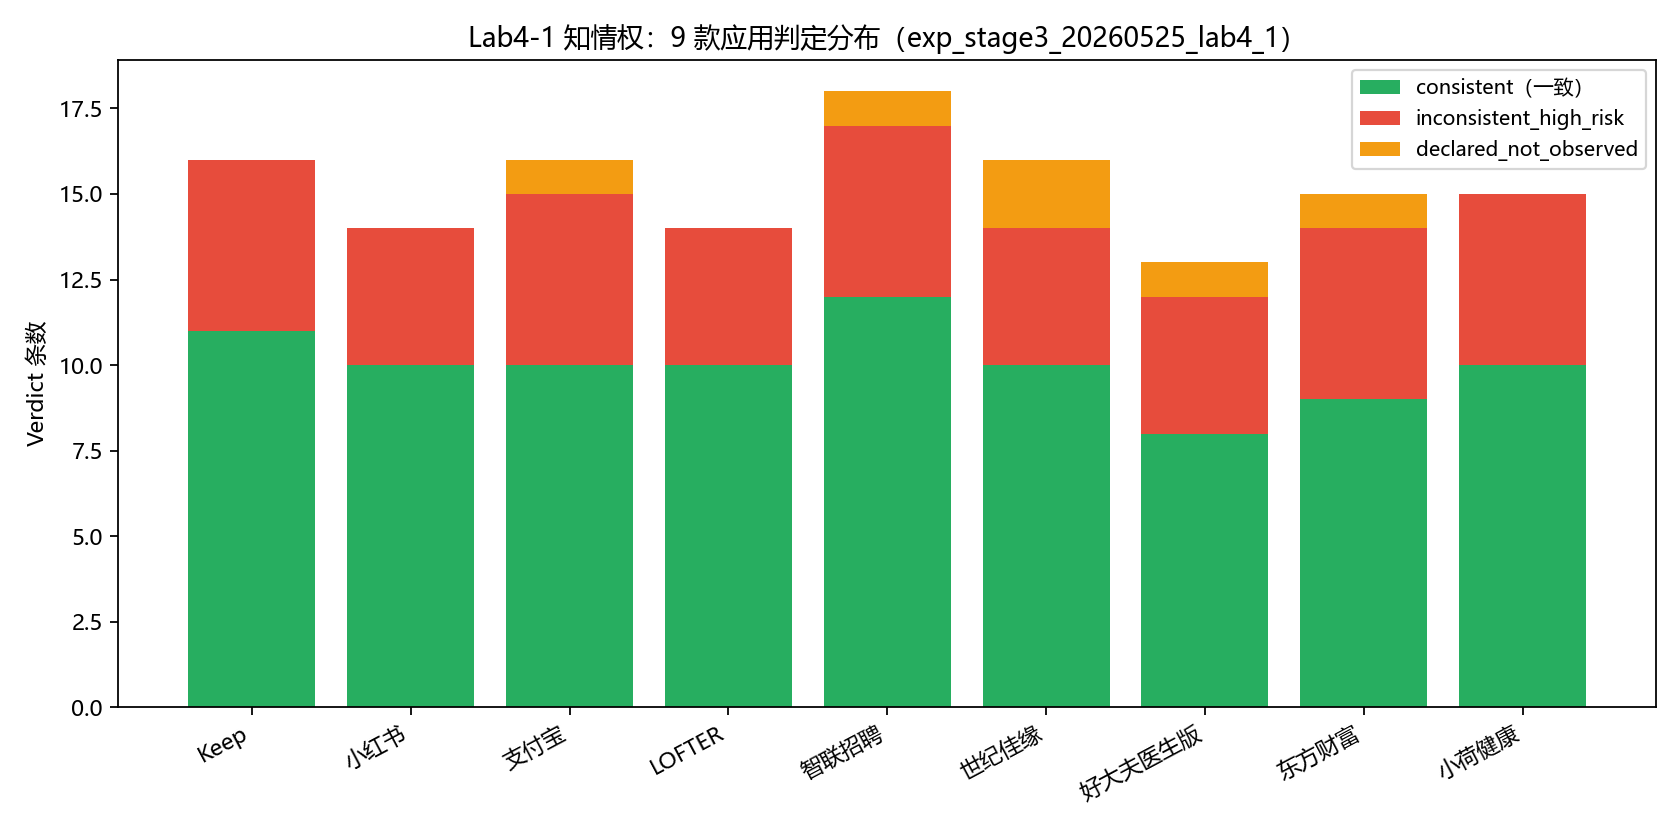
\includegraphics[width=0.95\linewidth]{fig_lab41_verdict_stacked.png}
\end{frame}

\begin{frame}
    \frametitle{Lab4-1 分 App 数据摘要}
    \tiny
    \begin{tabularx}{\textwidth}{|l|r|r|r|r|r|}
        \hline
        \textbf{App} & \textbf{声明} & \textbf{观测} & \textbf{一致} & \textbf{高风险} & \textbf{未观测} \\
        \hline
        Keep & 11 & 18 & 9 & 9 & 2 \\
        \hline
        小红书 & 12 & 18 & 10 & 8 & 2 \\
        \hline
        支付宝 & 12 & 18 & 10 & 8 & 2 \\
        \hline
        LOFTER & 12 & 18 & 10 & 8 & 0 \\
        \hline
        智联招聘 & 12 & 18 & 10 & 8 & 0 \\
        \hline
        世纪佳缘 & 12 & 18 & 10 & 8 & 0 \\
        \hline
        好大夫医生版 & 12 & 18 & 10 & 8 & 0 \\
        \hline
        东方财富 & 12 & 18 & 10 & 8 & 0 \\
        \hline
        小荷健康 & 12 & 18 & 10 & 8 & 0 \\
        \hline
    \end{tabularx}
    \scriptsize
    数据来源：\texttt{batch\_lab4-1\_exp\_stage3\_20260525\_lab4\_1\_summary.json}。
\end{frame}

\begin{frame}
    \frametitle{典型案例：高风险不一致}
    \small
    \begin{itemize}
        \item 现象：\texttt{observed\_count} 常大于 \texttt{declared\_count}（静态 SDK、历史审计、KB 推断并入观测集）。
        \item 解读：应用在政策中未充分声明的类型，在技术侧或知识库侧已有信号 $\rightarrow$ \texttt{inconsistent\_high\_risk}。
        \item 答辩话术：强调 \textbf{证据链分项}（static / oldsrc / kb / dynamic），避免笼统「Frida 抓到了」。
        \item 可展示单 App \texttt{<App>\_lab4\_1\_report.json} 中一条 \texttt{inconsistent\_high\_risk} 的 \texttt{sources}。
    \end{itemize}
\end{frame}

\begin{frame}
    \frametitle{Lab4-2 同意权（未完成有效实证）}
    \small
    \begin{itemize}
        \item 设计：对比「个性化推荐/隐私开关」关闭前、后 Frida 有效 API 命中。
        \item 实际：\texttt{before} 为本次真机包，\texttt{after} 多为 oldsrc derived；且无 \texttt{frida\_runtime\_events}。
        \item 结果：9/9 \texttt{report\_status\_failed}，\texttt{review\_needed}。
        \item 后续：关开关后 \textbf{二采} + 稳定 attach + 明确「有效事件」定义。
    \end{itemize}
\end{frame}

\begin{frame}
    \frametitle{Lab4-3 访问权（流水线成功 $\neq$ 合规结论）}
    \small
    \begin{itemize}
        \item 设计：\texttt{declared} vs \texttt{runtime\_observed\_pii} vs \texttt{lab4\_3\_copy} 字段覆盖。
        \item 实际：\texttt{lab4\_3\_copy} 来自 oldsrc \texttt{access\_result.json}（可用性测试字段）；非用户导出副本。
        \item 各 App \texttt{coverage\_rate = 0}，\texttt{runtime\_observed\_pii = []}。
        \item CLI 注意：\texttt{lab4-3-audit --dynamic-dir}（非 \texttt{--dynamic-evidence-dir}）。
    \end{itemize}
\end{frame}

\section{总结与展望}

\begin{frame}
    \frametitle{阶段性结论}
    \small
    \begin{itemize}
        \item 已完成 \textbf{工程化端到端流水线}：政策 $\rightarrow$ 静/动证据 $\rightarrow$ 合并 $\rightarrow$ Lab4 batch 报告。
        \item \textbf{主实验结论}来自 Lab4-1：9 App 可解释知情权审计，合计 90 条一致、41 条高风险不一致。
        \item Stage3 \textbf{UI 自动化}已覆盖 9 App 政策路径，并针对世纪佳缘、小荷等完成适配。
        \item 须在汇报中诚实说明：Frida 运行时事件为 0、Lab4-2 未过、Lab4-3 副本语义为历史可用性数据。
    \end{itemize}
\end{frame}

\begin{frame}
    \frametitle{后续工作}
    \small
    \begin{enumerate}
        \item 修复 Frida attach / hook，使 \texttt{frida\_runtime\_events} $>$ 0，支撑 Lab4-2。
        \item Lab4-2：关「个性化推荐」后二次 Stage3，形成真实 before/after 对比。
        \item Lab4-3：采集真实个人信息导出 JSON，替换 oldsrc 可用性字段。
        \item 可选：从 Lab4-1 挑 1--2 个 App 做口述案例 + 截图/报告片段展示。
    \end{enumerate}
\end{frame}

\begin{frame}
    \frametitle{复现与文档索引}
    \scriptsize
    \begin{itemize}
        \item 实验报告：\texttt{src/output/result/result\_20260525.md}
        \item 图表生成：\texttt{ppt/generate\_lab4\_ppt.py}
        \item 本 TeX：\texttt{ppt/lab4\_slide.tex}；PPTX：\texttt{ppt/系统设计Lab4.pptx}
        \item 编译：\texttt{xelatex lab4\_slide.tex}（需先生成 \texttt{figures\_lab4/}）
    \end{itemize}
\end{frame}

\begin{frame}
    \begin{center}
        {\Huge 感谢聆听！}\\[0.8em]
        {\large Q \& A}
    \end{center}
\end{frame}

\end{document}
